 %%%%% Fichero de ejemplo LaTeX que ilustra el uso de la Hoja de Estilo %%%%%%
%%%%% Jornadas.cls para Jornadas Sarteco

\documentclass[twocolumn,twoside]{Jornadas}
\usepackage{listings}
\usepackage[utf8]{inputenc}
\usepackage[spanish]{babel}
\usepackage{listings}
\usepackage{algorithm}
\usepackage{algorithmicx}
\usepackage{algcompatible}
\usepackage{adjustbox}
\usepackage{graphicx}
\usepackage{color}
\usepackage{caption}
\captionsetup{font=footnotesize}
\usepackage[caption=false,font=footnotesize]{subfig}
%\setlength{\marginparwidth}{2cm}
%\usepackage{todonotes}
\usepackage{placeins}
\usepackage{hyperref}
\usepackage{url}

% -*- Ajustes LaTeX en relación a las figuras -*-
\setcounter{topnumber}{10}     % Max. numero de figs. on top
\setcounter{bottomnumber}{10}  % Max. numero de figs. abajo
\setcounter{totalnumber}{10}   % Max. numero de figs. por pagina
\renewcommand{\topfraction}{1} % Max. fraccion de pagina ocupada por figs.
\renewcommand{\bottomfraction}{1}
\renewcommand{\textfraction}{0}  % Min. fraccion de pagina ocupada por texto
\renewcommand{\floatpagefraction}{1} % Max. espacio de pagina solo con figs.

\definecolor{gray97}{gray}{.97}
\definecolor{gray75}{gray}{.75}
\definecolor{gray45}{gray}{.45}

\lstset{
     inputencoding=utf8,
     extendedchars=true,
     backgroundcolor=\color{gray97},
     %
     stringstyle=\ttfamily,
     showstringspaces = false,
     basicstyle=\scriptsize\ttfamily,
     commentstyle=\color{gray45},
     keywordstyle=\bfseries,
     linewidth=.98\columnwidth,
     xleftmargin=3mm,
     breaklines=true,
     numbers=left,
     numbersep=6pt,
     numberstyle=\tiny,
     numberfirstline = false,
     firstnumber=auto,
     breaklines=true,
     %
     escapeinside={(*@}{@*)},
     literate={á}{{\'a}}1 {é}{{\'e}}1 {í}{{\'i}}1 {ó}{{\'o}}1 {ú}{{\'u}}1 {ñ}{{\~n}}1
   }

\def\BibTeX{{\rm B\kern-.05em{\sc i\kern-.025em b}\kern-.08em
    T\kern-.1667em\lower.7ex\hbox{E}\kern-.125emX}}

\newtheorem{theorem}{Teorema}

\hyphenation{pa-ra-le-lis-mo pro-cee-dings}

%Directorios en los que se buscan las figuras
\graphicspath{{.}{./Figuras/}}
%%%%%%%%%%%%%%%%%%%%%%%%%%%%%%%%%%%%%%%%%%%%

\begin{document}

\title{Analítica Prescriptiva}

\author{%
     Mendoza Mestanza Gutenberg Stiven%
     \thanks{Facultad de Ingeniería en Sistemas Informáticos, Ciencias de la Computación, e-mail: {\tt gutenberg.mendoza@epn.edu.ec}},
     Moya Barragán Fabricio Alejandro% 
     \thanks{Facultad de Ingeniería en Sistemas Informáticos, Ciencias de la Computación, 
     e-mail: {\tt fabricio.moya@epn.edu.ec}}
}

\maketitle
% Oculta las cabeceras y los números de página.
% Ambos elementos se añadirán durante la edición de las actas completas.
\markboth{}{}
\pagestyle{empty} 
\thispagestyle{empty} % Oculta el número de la primera página

\begin{abstract}
Este estudio presenta el desarrollo de un modelo predictivo basado en Árbol de decisión para clasificar el nivel de contaminación ambiental. Se utiliza la librería LazyPredict de Python para evaluar diferentes modelos y se analizan las métricas obtenidas. Se discuten las limitaciones identificadas y se sugieren trabajos futuros. Este enfoque puede contribuir a la toma de decisiones informadas y a la implementación de medidas de protección ambiental más efectivas.
.
\end{abstract}

\begin{keywords}
contaminación ambiental, modelado predictivo, Árbol de decisión, LazyPredict, clasificación.
\end{keywords}

%Añade los ficheros que necesites:

%!TEX root = main.tex
\section{Introducción}
La contaminación ambiental es un problema global que afecta la calidad de vida de las personas y el equilibrio ecológico del planeta. La capacidad de predecir y clasificar el nivel de contaminación en diferentes áreas geográficas es crucial para implementar medidas efectivas de mitigación y control. En este contexto, el modelado predictivo se presenta como una herramienta prometedora para abordar este desafío.\\

El objetivo de este estudio es desarrollar un modelo predictivo capaz de clasificar el nivel de contaminación en base a datos recopilados de diferentes fuentes y variables ambientales relevantes. Para lograrlo, se emplea la librería LazyPredict de Python, que permite evaluar diferentes modelos de clasificación y determinar cuál presenta la mejor exactitud en base a un conjunto de datos de muestra.\\

En este informe, se presenta el proceso de modelado predictivo realizado utilizando un modelo basado en Árbol de decisión (DecisionTreeClassifier) y se analizan las métricas obtenidas para evaluar su desempeño. Asimismo, se explora la utilización de la validación cruzada para obtener una evaluación más robusta del modelo.\\

Las limitaciones identificadas durante el estudio y las sugerencias de trabajos futuros se discuten con el fin de mejorar y ampliar el modelo predictivo en futuras investigaciones. En última instancia, se espera que este estudio contribuya al desarrollo de herramientas efectivas para la clasificación y predicción del nivel de contaminación, permitiendo tomar decisiones informadas y implementar medidas de protección ambiental más eficientes.\\

\input{Papper IB/02-Definición_del_problema}
%!TEX root = main.tex
\section{Preprocesamiento de datos}

En nuestra primera etapa de preprocesamiento de datos, nos embarcamos en un análisis de dimensionalidad de múltiples conjuntos de datos con estructuras similares. Este análisis nos permitió determinar que todos los conjuntos de datos eran estructuralmente idénticos, lo que significa que el análisis de un conjunto de datos individual sería representativo del análisis de todos los conjuntos juntos. A continuación, desarrollamos una función para calcular el Índice de Calidad del Aire (AQI) basándonos en los contaminantes presentes y lo separamos en cuatro categorías distintas: Excellent - Good, Slightly - Lightly Polluted, Moderately - Heavily Polluted, y Severely Polluted.\cite{liang2015beijing}

Empleamos la correlación de Pearson para identificar correlaciones dentro de los datos, y establecimos un umbral de 0.8 para eliminar aquellas columnas que exhibían una alta correlación. Este proceso nos permitió minimizar la redundancia y mejorar la eficiencia del modelo que estamos entrenando. 

A continuación, abordamos la presencia de valores nulos en los conjuntos de datos. Para la mayoría de las columnas, reemplazamos estos valores con la media. Sin embargo, para la columna 'wd', implementamos una técnica llamada codificación 'dummy' o 'one-hot'. En el caso de las columnas 'station' y 'AQI', aplicamos codificación de etiquetas (label encoding) para convertir los datos categóricos en una forma que nuestro modelo de aprendizaje automático podría interpretar y procesar.

Para finalizar, equilibramos nuestro conjunto de datos utilizando la técnica RandomOverSampler, lo cual ayuda a evitar un sesgo hacia clases más frecuentes. Este proceso de preprocesamiento es esencial para preparar nuestros datos para la formación del modelo de aprendizaje automático.\cite{liang2014hourly}

%!TEX root = main.tex
\section{Análisis exploratorio de datos}

El \href{https://www.ibm.com/es-es/cloud/learn/exploratory-data-analysis}{análisis exploratorio de datos} es un proceso que permite conocer a priori la naturaleza de los conjuntos.

El análisis exploratorio de datos (AED) es una etapa crucial en la investigación y el análisis de datos. Su objetivo es comprender la estructura y las características de un conjunto de datos antes de aplicar técnicas estadísticas más avanzadas o construir modelos predictivos. El AED ayuda a identificar patrones, tendencias, valores atípicos y relaciones entre variables, lo que permite formular hipótesis y generar conocimientos preliminares sobre los datos, respondiendo así algunas preguntas como: 

\begin{enumerate}
    \item ¿Cuál es la distribución de las variables en el conjunto de datos?
    \item ¿Existen correlaciones entre las variables?
    \item ¿Hay valores atípicos que necesiten ser investigados?
    \item ¿Cuáles son las características más relevantes o distintivas del conjunto de datos?
    \item ¿Hay patrones o tendencias interesantes que se puedan identificar?
\end{enumerate}

En particular en esta ocasión nos permite obtener algunas posibles conclusiones:

\begin{enumerate}
    \item \textbf{Patrones temporales:} Al analizar los datos a lo largo del período de tiempo (del 1 de marzo de 2013 al 28 de febrero de 2017), es posible identificar patrones temporales en la contaminación del aire. Esto puede revelar estacionalidades, tendencias a largo plazo y variaciones interanuales en la calidad del aire en Beijing.
    \item \textbf{Variaciones geográficas:} Al tener datos de 12 sitios de monitoreo de calidad del aire en Beijing, es posible analizar las variaciones geográficas en los niveles de contaminantes. Esto puede revelar áreas específicas que son más susceptibles a altos niveles de contaminación o identificar diferencias significativas en la calidad del aire entre diferentes partes de la ciudad.
    \item \textbf{Correlaciones entre contaminantes:} Al analizar los datos de los cinco contaminantes atmosféricos (SO2, NO2, PM10, CO y O3), se pueden identificar correlaciones y relaciones entre ellos. Por ejemplo, es posible que se encuentre una correlación positiva entre los niveles de NO2 y PM10, lo que sugiere que ciertos contaminantes están relacionados entre sí.
    \item \textbf{Influencia de los factores meteorológicos:} Al relacionar los datos de calidad del aire con los datos meteorológicos de la estación más cercana, se puede investigar la influencia de los factores meteorológicos en la contaminación del aire. Esto puede revelar cómo variables como la temperatura, la humedad, la velocidad del viento, etc, pueden afectar los niveles de contaminantes y proporcionar información útil para comprender los factores que contribuyen a la calidad del aire en Beijing.
    \item \textbf{Interpretación del Índice de Calidad del Aire (AQI):} Al comprender cómo se calcula y se interpreta el Índice de Calidad del Aire (AQI) en función de los cinco contaminantes atmosféricos mencionados (SO2, NO2, PM10, CO y O3), se puede proporcionar una interpretación más detallada y precisa de la calidad del aire en diferentes días y contextos.
\end{enumerate}

El objetivo es obtener una comprensión más profunda de la calidad del aire en Beijing, identificar patrones y relaciones clave, y proporcionar información útil para futuras investigaciones y medidas de control de la contaminación o en el desarrollo de modelos.\cite{liang2016spatiotemporal}

\begin{figure}[htb] 
    \begin{center} 
        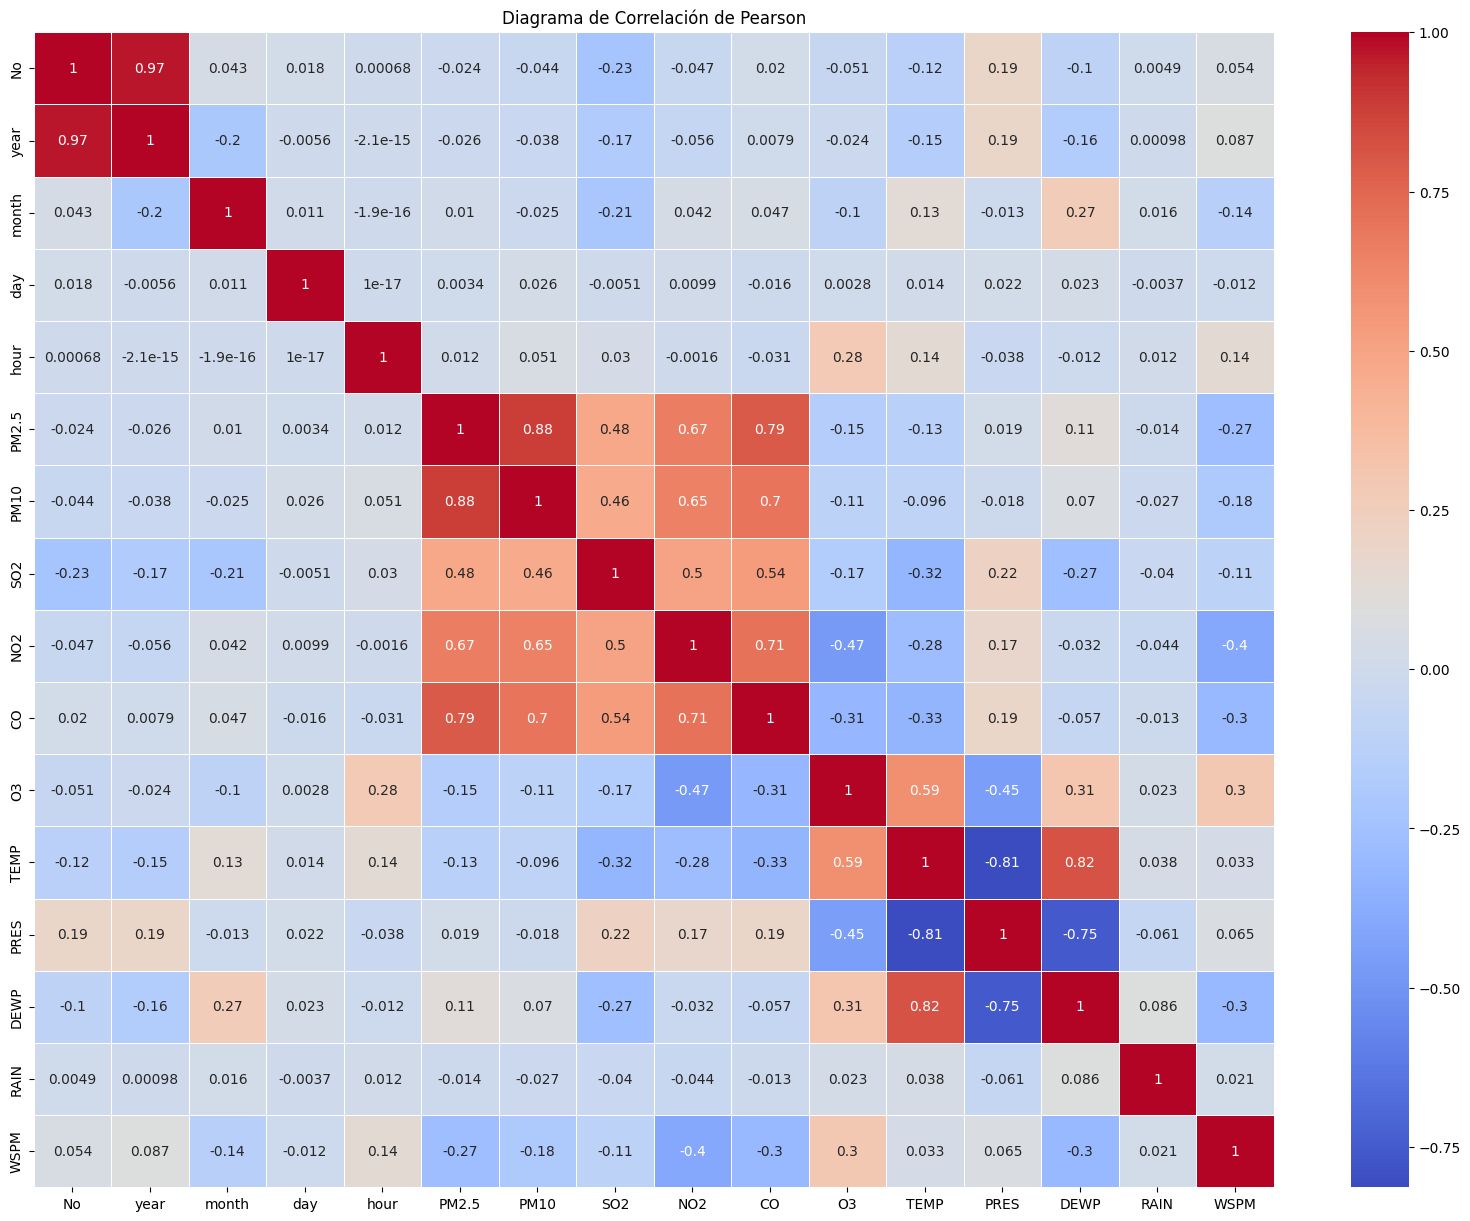
\includegraphics[width=8cm]{Papper IB/Images/correlation_matrix.png}
    \end{center} 
    \caption{Matriz de Correlación de Pearson.} 
    \label{fig:fig1} 
\end{figure} 

Informe: Análisis de correlaciones en el conjunto de datos de calidad del aire de Beijing

La matriz de correlación de Pearson se usa con el objetivo de comprender las correlaciones entre las variables y proporcionar una visión más profunda de la contaminación del aire en Beijing, se presentan los hallazgos clave derivados del análisis de correlaciones.

\subsection{\textbf{Correlación positiva fuerte}}
Se observó una correlación positiva fuerte (0.884380) entre los niveles de partículas suspendidas de diámetro menor a 2.5 micrómetros (PM2.5) y los niveles de partículas suspendidas de diámetro menor a 10 micrómetros (PM10). Esta correlación indica que los niveles de partículas PM2.5 están altamente correlacionados con los niveles de partículas PM10. Es importante tener en cuenta que las partículas PM2.5 son un subconjunto de las partículas PM10.

\subsection{\textbf{Correlaciones positivas moderadas}}
Se encontraron correlaciones positivas moderadas entre los niveles de partículas PM2.5 y los niveles de monóxido de carbono (CO) (0.789998) y dióxido de nitrógeno (NO2) (0.666948). Estas correlaciones sugieren que los niveles de partículas suspendidas de diámetro menor a 2.5 micrómetros están relacionados con la presencia de CO y NO2 en el aire. Esto indica que la presencia de CO y NO2 puede contribuir a la contaminación del aire por partículas PM2.5.

\subsection{\textbf{Correlación negativa moderada}}
Se encontró una correlación negativa moderada (-0.349856) entre los niveles de dióxido de azufre (SO2) y los niveles de dióxido de nitrógeno (NO2). Esta correlación inversa indica que los niveles de SO2 y NO2 en el aire tienden a tener una relación inversa. Es importante considerar esta relación en el contexto de la calidad del aire, ya que la presencia de estos contaminantes puede tener diferentes fuentes y efectos en la salud y el medio ambiente.

\subsection{\textbf{Correlación con variables meteorológicas}}
Se observaron correlaciones débiles a moderadas entre las variables de contaminantes atmosféricos (PM2.5, PM10, SO2, NO2, CO, O3) y las variables meteorológicas (TEMP, PRES, DEWP, RAIN, WSPM). Estas correlaciones indican que los factores meteorológicos pueden influir en los niveles de contaminantes en el aire. Por ejemplo, la temperatura (TEMP) puede estar relacionada con la formación de ozono (O3), y la velocidad del viento (WSPM) puede afectar la dispersión de los contaminantes. Sin embargo, es importante destacar que estas correlaciones son de naturaleza débil a moderada y se requiere un análisis más profundo para comprender plenamente la influencia de los factores meteorológicos en la contaminación del aire.

En conclusión, el análisis de correlaciones ha proporcionado información valiosa sobre las relaciones entre las variables. Estas correlaciones destacan la fuerte relación entre las partículas PM2.5 y PM10, así como las asociaciones moderadas entre los contaminantes atmosféricos y los factores meteorológicos. Estos hallazgos contribuyen a una mejor comprensión de los factores y pueden servir como base para investigaciones posteriores y medidas de control de la contaminación atmosférica en la región.\cite{liang2017comparison}

\subsection{\textbf{Simetría de los datos}}
Se analizó la diferencia entre la media y la mediana de las variables numéricas en el conjunto de datos, con el fin de obtener información sobre la simetría de la distribución de los datos y la presencia de valores atípicos. 

\begin{itemize}
    \item \textbf{Diferencias nulas:} Se observó que las variables "No" y "hour" presentan una diferencia de cero entre la media y la mediana. Esto indica que no hay una discrepancia significativa entre estos valores estadísticos para dichas variables. En otras palabras, la distribución de los datos para estas variables es simétrica.
    \item \textbf{Diferencias negativas:} Las variables "year", "month", "day", "TEMP" y "DEWP" mostraron diferencias negativas entre la media y la mediana. Estas diferencias sugieren que estas variables tienden a tener una distribución asimétrica hacia la izquierda. Es decir, la concentración de valores más bajos arrastra la media hacia abajo en comparación con la mediana.
    \item \textbf{Diferencias positivas:} Por otro lado, se encontró que las variables "PM2.5", "PM10", "SO2", "NO2", "CO", "O3", "PRES", "RAIN" y "WSPM" presentaron diferencias positivas entre la media y la mediana. Esto indica que estas variables tienden a tener una distribución asimétrica hacia la derecha. En otras palabras, la presencia de valores más altos influye en la media y la aleja de la mediana.
\end{itemize}

\begin{figure}[htb] 
    \begin{center} 
        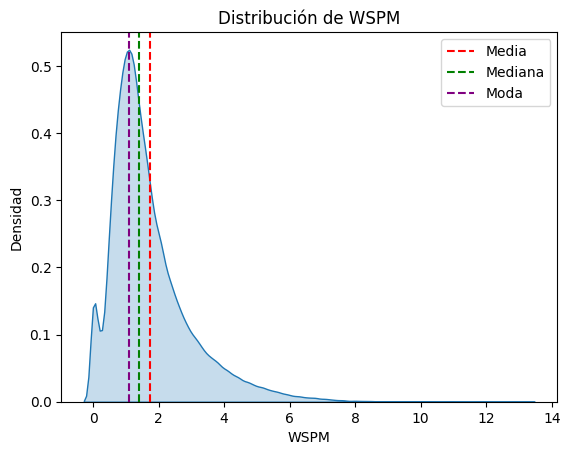
\includegraphics[width=8cm]{Papper IB/Images/simetria_wspm.png}
    \end{center} 
    \caption{Simetría WSPM.} 
    \label{fig:fig1} 
\end{figure} 

Es importante tener en cuenta que estas diferencias entre la media y la mediana son indicadores de la distribución de los datos y pueden sugerir la presencia de valores atípicos o asimetría en los conjuntos de datos correspondientes a cada variable.

\subsection{Tendencias y variaciones}
Obtener gráficos de puntos que representen la mediana de diferentes variables relacionadas con la calidad del aire, como PM2.5, PM10, SO2, NO2, CO, O3, entre otras, en función de los meses y los años.

\begin{figure}[htb] 
    \begin{center} 
        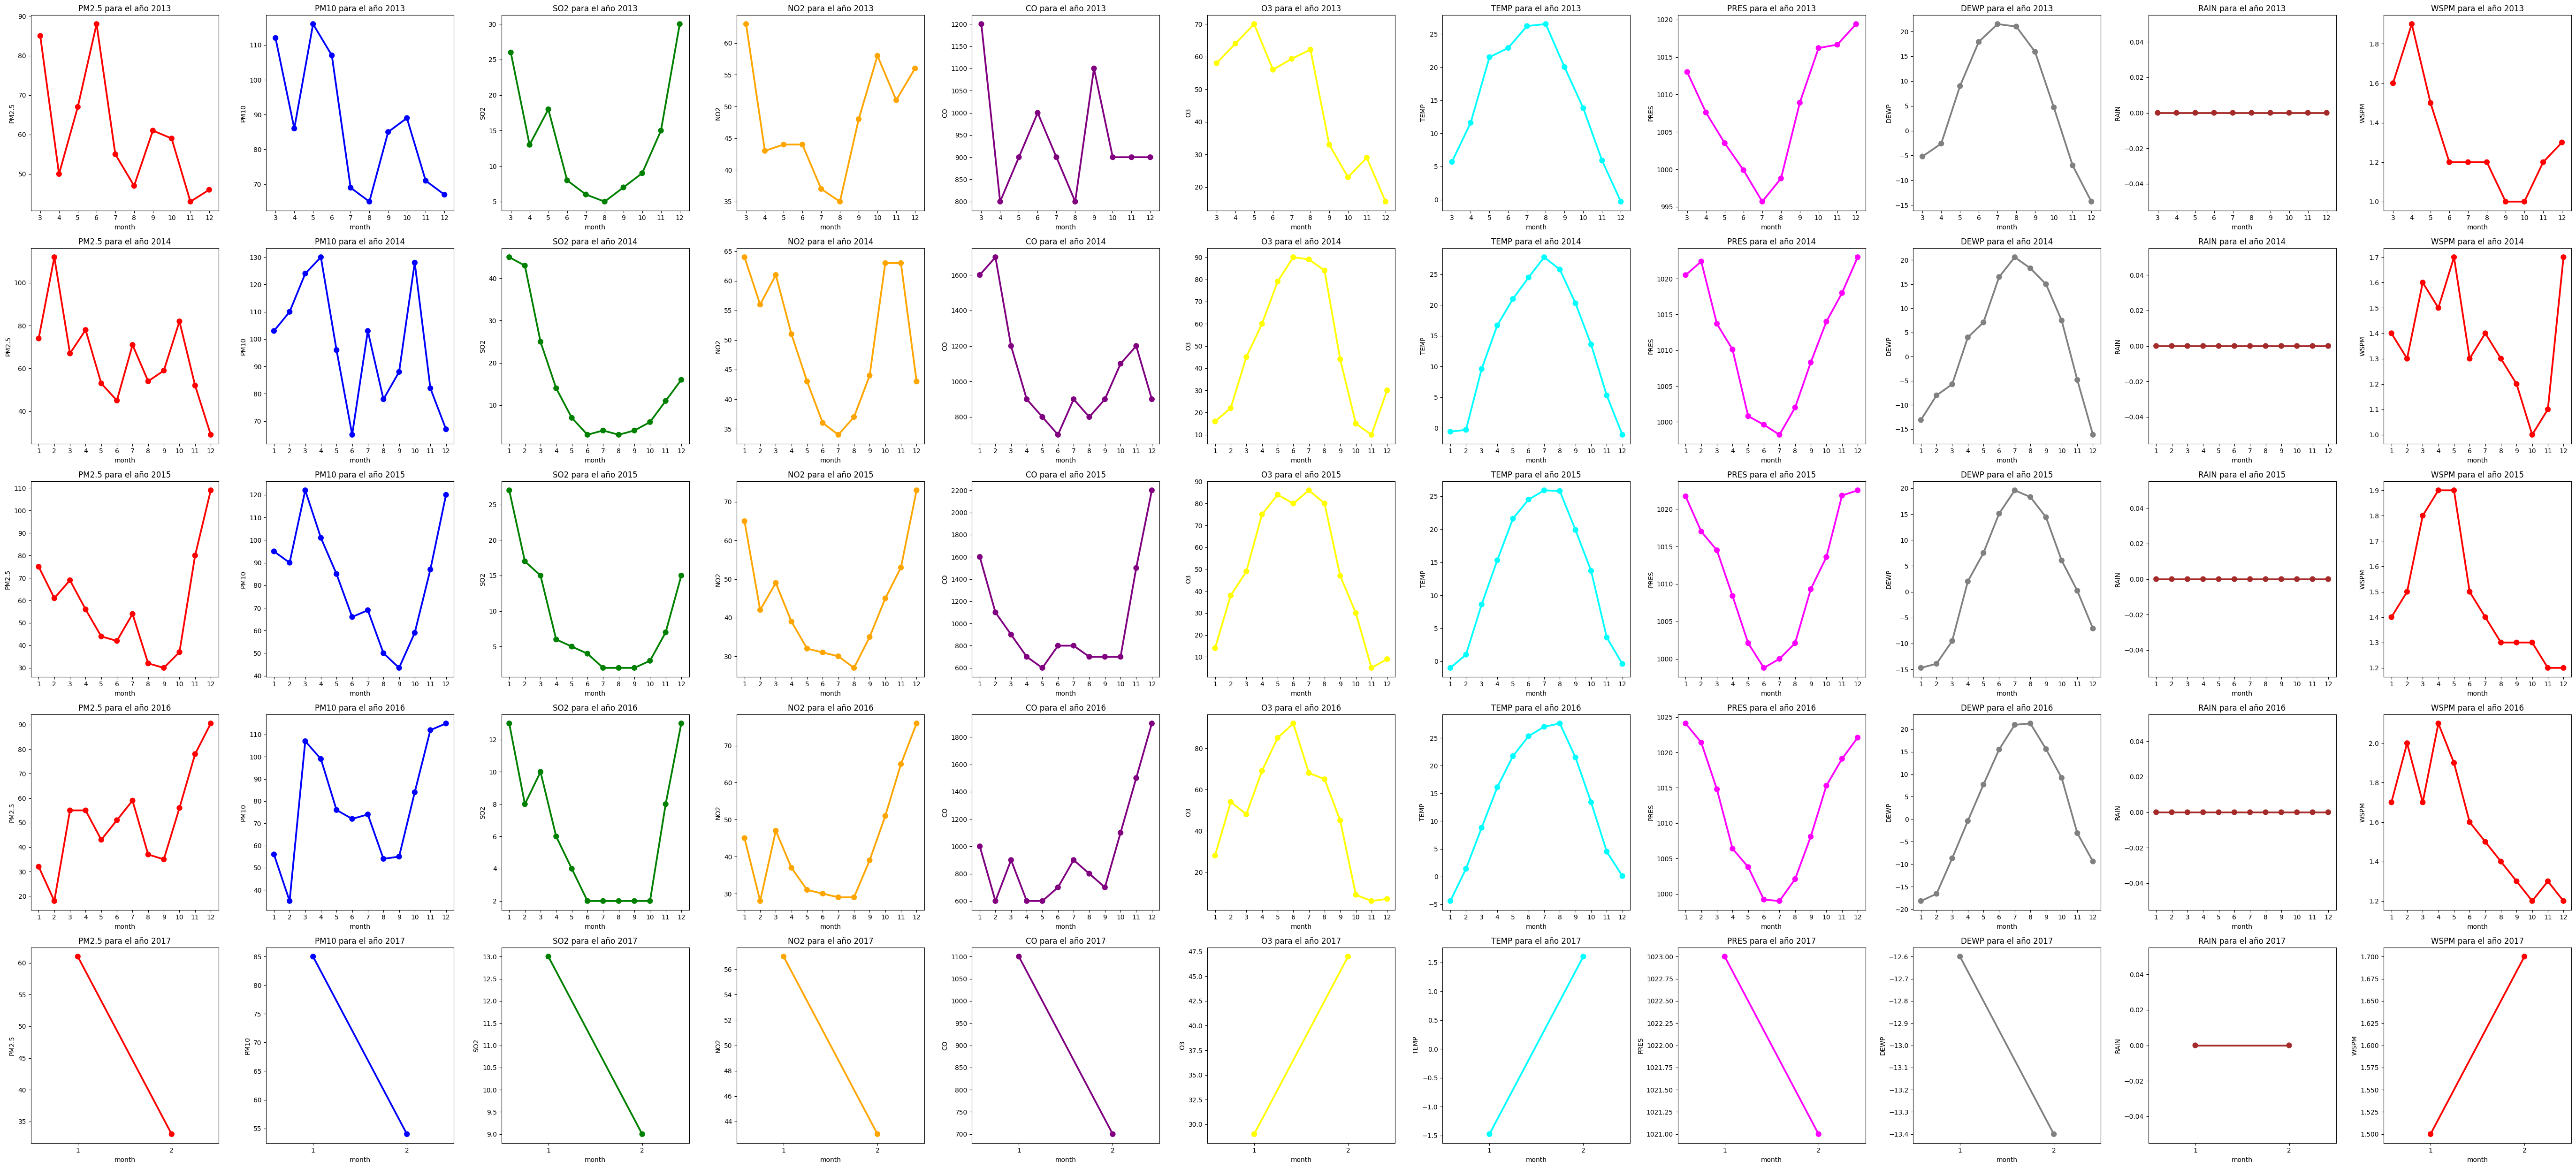
\includegraphics[width=8cm]{Papper IB/Images/expands_all_years.png}
    \end{center} 
    \caption{Simetría WSPM.} 
    \label{fig:fig1} 
\end{figure} 

El análisis permite una exploración visual detallada de la calidad del aire en Beijing a lo largo de los años y los meses. Esto proporcionaría información clave sobre patrones estacionales, cambios a largo plazo y eventos excepcionales en la calidad del aire en la región, lo que sería fundamental para comprender y abordar los desafíos relacionados con la contaminación atmosférica.\cite{liu2018spatio}

El análisis exploratorio de datos es un proceso iterativo, y es posible que nuevas preguntas e hipótesis surjan a medida que se profundiza en los datos y se descubren nuevas perspectivas.
\section{Modelado predictivo}

En esta sección, se presenta el modelado predictivo realizado para clasificar los datos según el nivel de contaminación. Para ello, se empleó la librería de Python LazyPredict\cite{LazyPredict}, la cual nos permitió identificar qué modelo presenta la mejor exactitud sobre un conjunto de datos de muestra.

\begin{figure}[htb] 
    \begin{center} 
        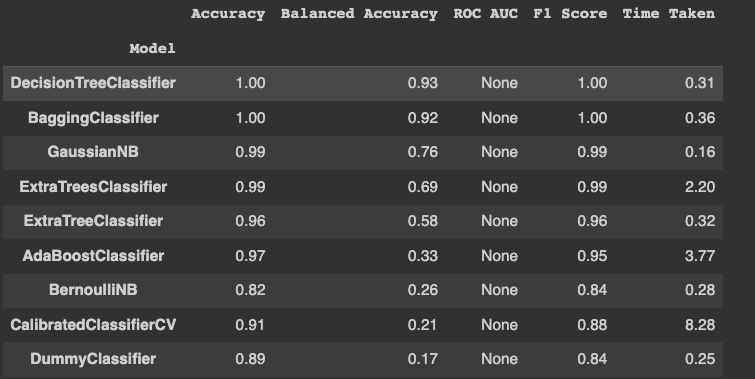
\includegraphics[width=8cm]{Papper IB/Images/model_1.png}
    \end{center} 
    \caption{Salida de LazyPredictor} 
    \label{fig:fig4} 
\end{figure} 

El análisis de LazyPredictor nos indica que se recomienda utilizar un modelo basado en Árbol de decisión (DecisionTreeClassifier). A continuación, se procedió a entrenar el modelo utilizando este algoritmo y posteriormente se analizaron las métricas obtenidas.

El modelo fue entrenado inicialmente sin especificar los hiperparámetros del Árbol de decisión, tales como max\_depth, min\_samples\_leaf y min\_samples\_split. Los resultados obtenidos se muestran en la siguiente figura:

\begin{figure}[htb] 
    \begin{center} 
        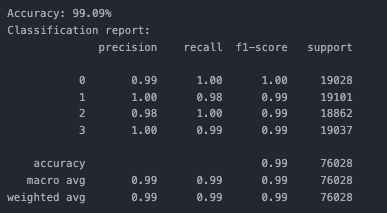
\includegraphics[width=8cm]{Papper IB/Images/model_2.png}
    \end{center} 
    \caption{Reporte de clasificación} 
    \label{fig:fig2} 
\end{figure} 

A partir de los resultados presentados en el reporte, se pueden extraer diversas conclusiones relevantes.

En primer lugar, el modelo obtuvo una precisión del 99.09\%, lo cual indica que fue capaz de clasificar correctamente el 99.09\% de las instancias en el conjunto de datos. Esta alta precisión evidencia la capacidad del modelo para realizar una clasificación confiable del nivel de contaminación.\cite{xu2017long}

El reporte de clasificación también incluye métricas como recall y F1-Score para cada clase. Estas métricas proporcionan información adicional sobre la capacidad del modelo para identificar correctamente las instancias positivas y negativas. En general, se observa que el modelo obtuvo valores elevados de recall y F1-Score para todas las clases. Esto indica que el modelo logró identificar la mayoría de las instancias reales de cada clase y alcanzó un equilibrio entre precisión y recall.\cite{liang2018analysis}

Además, es relevante destacar que el modelo fue evaluado en un conjunto de datos de considerable tamaño, con un total de 76,028 instancias. Esta cantidad de datos aumenta la confianza en los resultados y sugiere que el modelo ha sido probado en un escenario realista.

\subsection{Validación cruzada}

La validación cruzada es una técnica esencial para evaluar el rendimiento del modelo de manera robusta. En este caso, se realizó una validación cruzada y se obtuvieron los siguientes datos:

\textbf{Mejores parámetros:}
\begin{itemize}
    \item max\_depth: None
    \item min\_samples\_leaf: 1
    \item min\_samples\_split: 2
\end{itemize}

\textbf{Puntuaciones de validación cruzada:}
\begin{itemize}
    \item [0.99019166, 0.98928974, 0.99036077, 0.99007892, 0.99024803, 0.99126268, 0.99013473, 0.99086758, 0.98945826, 0.98844354]
\end{itemize}

\textbf{Puntuación promedio de validación cruzada:} 0.990033590214823

\textbf{Exactitud:} 99.10\%

Estos resultados confirman y respaldan el desempeño del modelo de Árbol de decisión en la clasificación del nivel de contaminación. La obtención de una puntuación promedio de validación cruzada alta indica que el modelo es consistente y generaliza bien en diferentes subconjuntos de datos, esto también se puede evidenciar en la matriz de confusión\\ 
\begin{figure}[htb] 
    \begin{center} 
        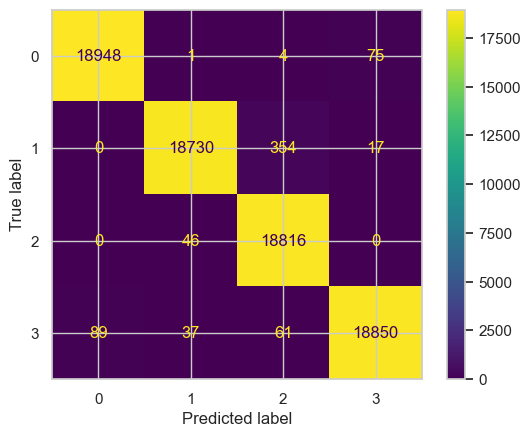
\includegraphics[width=8cm]{Papper IB/Images/model_3.png}
    \end{center} 
    \caption{Matriz de confusión} 
    \label{fig:fig2} 
\end{figure} 


En conclusión, el modelo de Árbol de decisión ha demostrado ser altamente efectivo en la clasificación del nivel de contaminación. Los resultados obtenidos, respaldados por las métricas de evaluación y la validación cruzada, indican que el modelo es confiable y preciso en su capacidad para clasificar correctamente el nivel de contaminación en función de los datos proporcionados. Estos resultados son alentadores y sugieren la aplicabilidad del modelo en situaciones reales relacionadas con la clasificación de la contaminación.\cite{li2017study}

Finalmente una metrica muy importante es comprender si el modelo tiene overfitting o underfitting, eso se puede visualizar en la siguiente grafica: 
\begin{figure}[htb] 
    \begin{center} 
        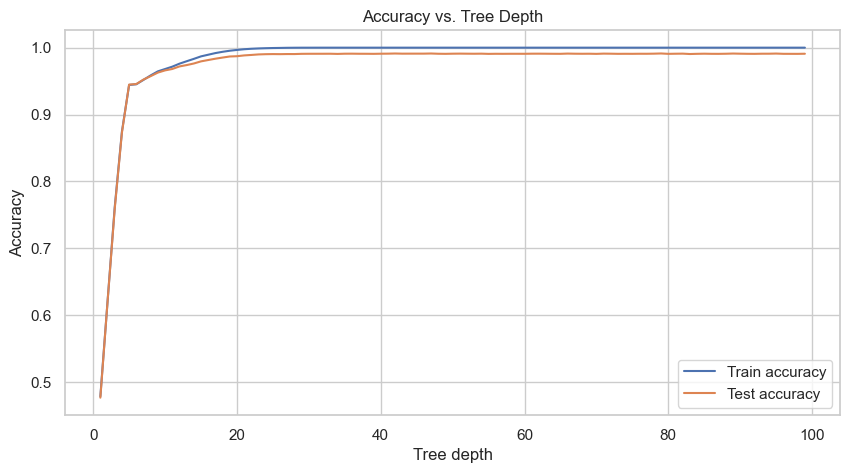
\includegraphics[width=8cm]{Papper IB/Images/model_4.png}
    \end{center} 
    \caption{Matriz de confusión} 
    \label{fig:fig1} 
\end{figure} 

%!TEX root = main.tex
\section{Conclusiones}

En este estudio, se desarrolló un modelo predictivo utilizando la librería LazyPredict de Python y se obtuvieron resultados satisfactorios en la clasificación del nivel de contaminación. El modelo de Árbol de decisión alcanzó una precisión del 99.09\%, logrando clasificar correctamente la mayoría de las instancias en el conjunto de datos. 

El reporte de clasificación mostró valores elevados de recall y F1-Score para todas las clases, indicando una buena capacidad del modelo para identificar correctamente las instancias positivas y negativas. Además, el modelo fue evaluado en un conjunto de datos de tamaño considerable, lo que aumenta la confianza en su rendimiento.

Si bien existen limitaciones en cuanto al tamaño del conjunto de datos y la dependencia lineal asumida por el modelo de Árbol de decisión, los resultados obtenidos son alentadores y sugieren que el modelo puede ser útil en la clasificación del nivel de contaminación.

En cuanto a los trabajos futuros, se recomienda la recopilación de datos adicionales, la exploración de otros algoritmos de clasificación y el uso de enfoques de aprendizaje automático más avanzados para mejorar la precisión del modelo.

En resumen, este estudio demuestra la viabilidad de utilizar técnicas de modelado predictivo para la clasificación del nivel de contaminación. Los resultados obtenidos y las sugerencias de trabajos futuros pueden ser útiles para mejorar y ampliar el alcance de este enfoque en futuras investigaciones.


%!TEX root = main.tex
\section{Limitaciones}

A pesar de los buenos resultados obtenidos en el modelado predictivo para clasificar el nivel de contaminación, es importante tener en cuenta algunas limitaciones:

\begin{itemize}
    \item \textbf{Tamaño del conjunto de datos:} Aunque se trabajó con un conjunto de datos de tamaño considerable, es posible que un conjunto de datos aún más grande pudiera haber proporcionado resultados más robustos y precisos.
    \item \textbf{Dependencia de los datos de entrada:} El modelo de Árbol de decisión utilizado en este estudio asume una dependencia lineal entre las características de entrada y la variable objetivo. Sin embargo, en la realidad, la relación puede ser más compleja y no lineal, lo que podría afectar la precisión del modelo.
    \item \textbf{Falta de características relevantes:} Es posible que el conjunto de datos utilizado no incluya todas las características relevantes para predecir el nivel de contaminación de manera óptima. La adición de más características podría mejorar aún más el rendimiento del modelo.
\end{itemize}

%!TEX root = main.tex
\section{Trabajos Futuros}

Basado en las limitaciones identificadas y los resultados obtenidos, se sugieren posibles trabajos futuros para mejorar el modelado predictivo del nivel de contaminación:

\begin{itemize}
    \item \textbf{Recopilación de datos adicionales:} Se podría realizar una recopilación de datos más extensa, incluyendo una mayor variedad de características relevantes para el nivel de contaminación. Esto permitiría construir modelos más completos y precisos.
    \item \textbf{Explorar otros algoritmos de clasificación:} Además del Árbol de decisión, se podrían explorar otros algoritmos de clasificación y comparar su rendimiento con el modelo actual. Esto podría revelar si otro algoritmo puede ofrecer mejores resultados en términos de precisión y generalización.
    \item \textbf{Considerar enfoques de aprendizaje automático más avanzados:} Se podrían aplicar técnicas de aprendizaje automático más avanzadas, como el uso de redes neuronales o algoritmos de aprendizaje profundo, para mejorar la precisión de la clasificación del nivel de contaminación.
\end{itemize}

%!TEX root = main.tex
\section{Anexos}

\href{https://github.com/Afkerian/Beijing-Multi-Site-Air-Quality-Data-Data-Set}{Proyecto 02 del 1er Bimestre - GITHUB}


%\section*{Agradecimientos}

%%%El presente trabajo tiene como objetivo cumplir los requerimiento de la materia de Multiprocesamiento y Arquitecturas Alternativas, aplicando lo aprendido durante el semestre con el fin de plantear una propuesta viable de un Centro de Datos o Data Center que estaría ubicado en el campus "Ruber Orellana" de la Escuela Politécnica Nacional y cumpliría con las especificaciones de un programa de inclusión digital, permitiendo así a los estudiantes, docentes y planta científica desarrollar su investigación, siendo este Data Center de tipo TIER II. 

%Comenta la línea \nocite para que sólo se incluyan en las referencias
%las entradas que esté referenciadas en el texto con \cite{}
%\nocite{*}
\bibliographystyle{Jornadas}
\bibliography{biblio}

\end{document}

